\documentclass[conference,flushend]{iaria} % (based on IEEEtran.cls)
% The class iaria.cls loads biblatex/biber with correct IARIA settings
% as well as a set of common packages (times, inputenc[utf8], fontenc[T1],
% graphicx, xcolor, url, orcidlink, hyperref, extdash[shortcuts])

\usepackage{subfigure}
\usepackage{csquotes}
\usepackage{svg}
\usepackage{float}

% prevent overflowing URLs in bibliography
\usepackage{xurl}

\DeclareFieldFormat*{url}{}
\DeclareFieldFormat[misc]{url}{\mkbibacro{URL}\addcolon\space\url{#1}}
\DeclareFieldFormat*{urldate}{}
\DeclareFieldFormat[misc]{urldate}{\mkbibparens{\bibstring{urlseen}\space#1}}

\addbibresource{references.bib}
\title{Fast Charging Communication and Cybersecurity: A Technology Review}
\author{
  \IEEEauthorblockN{%
    Jakob Löw\orcidlink{0009-0006-7088-8684}, Kevin Mayer\orcidlink{0000-0002-5597-3913}, Hans-Joachim Hof\orcidlink{0000-0002-6930-9271}}
  \IEEEauthorblockA{%
    CARISSMA Institute of Electric, Connected and Secure Mobility \\
    University of applied sciences Ingolstadt \\
    Ingolstadt, Germany \\
    e-mail: {\tt$\lbrace$jakob.loew\,|\,kevin.mayer\,|\,hof$\rbrace$@thi.de}
} }
\begin{document}
\maketitle
\begin{abstract}
With the increasing amounts of electric vehicles on the road, the demand for public charging stations increases as well.
While AC charging is used for charging at home, DC fast charging is commonly used when traveling long distances.
Since DC fast charging requires higher level communication between vehicle and charging station, it provides an increased attack surface to both sides.
This paper reviews communication standards and their implementations used in fast charging scenarios.
Focusing on the cybersecurity aspects of these communications, we review and sketch up new mechanisms for attacking charging station communication.
\end{abstract}
\begin{IEEEkeywords}
charging; fast charging; ccs; iso15118; DC charging; electric vehicle; vehicle charging.
\end{IEEEkeywords}

\section{Introduction}
Many countries are currently transitioning away from combustion engine vehicles towards battery electric ones.
This transition is happening at a rapid rate, because buying an electric vehicle often gets incentivised through tax reductions or straight refunds \cite{kraftfahrtbundesamt_anzahl_2024}.
With people buying more and more electric vehicles, the demand for charging infrastructure rises.
In Germany not only electric vehicles, but also the buildup of charging infrastructure got heaviliy subsidized by the government.
This high demand and government incentives resulted in a rapid growth in charging station numbers, suppliers and operators \cite{bundesnetzagentur_anzahl_2024}.
Due to the rushed development, the cybersecurity of current charging stations is below average compared to other cyberphysical systems \cite{nasr_power_2022, johnson_review_2022, ahalawat_security_2022}.
Recently cybersecurity researchers investigating charging backend infrastructure have found a range of textbook vulnerabilities, such as SQL injection, cross site scripting or unauthenticated remote update procedures \cite{nasr_power_2022}.
\\
This paper will focus on fast charging stations. Because of their functional design, described in section \ref{sec:highlevelcomm}, they have a demand for complex two-way communication with the vehicle for exchanging charging conditions and limits.
While other works such as Tu et al. \cite{tu_extreme_2019} have already covered eletrical and other aspects of fast charging stations, this paper will focus on communication aspects.
The ISO15118 standard was created for communication between charging stations and vehicles, enabling interoperability between stations and vehicles from different manufacturers.
This high level communication protocol provides a larger attack surface compared to other charging techniques, making it more interesting for cybersecurity reserarch.
% TODO add outline of following sections

\section{Charging Station Communication}
Electricity generally comes in two forms: alternating current (AC) and direct current (DC).
While power grids are usually AC, batteries need to be charged using DC.
Therefore, the AC needs to be converted to DC either in the car or in the charging station itself.
While cars usually come with an onboard AC to DC converter for charging the onboard battery, their power is usually limited to 7 to 22 kW.
In order to achieve higher charging powers, a fast charging station provides a stationary AC to DC converter. Placing it outside of the car removes weight requirements, simplifies cooling and thus allows higher charging currents. \\
In general charging stations can be divided into three categories:
\begin{enumerate}
\item Unmetered AC charging (often used in residential buildings)
\item Commercial AC charging stations
\item DC fast charging stations
\end{enumerate}%
%
The following subsections describe the communication and payment mechanisms of these three kinds of charging stations as well as the included security concepts.

\subsection{Low Level Communication}
AC charging stations usually supply grid power directly, making them just sockets with some very basic communication to the vehicle.
In the early days of electric vehicle adoption mainly these kind of charging stations were built.
Because charging a modern vehicle using an AC charging station can take multiple hours, they usually aren't used for long distance driving.
Because of their low price and low electrical requirements they are however still widely used and newly installed, especially for home and office charging as well as on park and ride parking lots. \\
The by far most common plug for AC charging is the type 2 connector shown in figure \ref{fig:type2}. It is used not only the standard charging plug in Europe, but also in China and other parts of Asia.
Apart from the typical connections of a 3-phase power socket, the connector incorporates two additional pins: charge pilot (CP) and proximity pilot (PP).
These two pins are used for a very simple resistor based signaling scheme defined in IEC 61851 \cite{iec_iec_2010} and explained by \cite{dalheimer_ladeinfrastruktur_2017}:
The charging cable includes a resistor between proximity pilot and protective earth (PE), which signals the maximum current for this cable.
The charging station supplies a +12V/-12V pulse width modulation (PWM) signal between CP and PE.
The vehicle contains both a diode and a resistor between CP and PE, such that the charging station can detect the presence of a vehicle based on the negative voltage being dropped by the diode and the positive voltage being reduced by the resistor.
As soon as the vehicle is ready to charge it connects a second resistor between CP and PE further reducing the voltage.
For unmetered AC charging this is sufficient to start a charging session.
For public AC charging infrastructure usually external means of payment, such as mobile app activation or contactless payment have to be used before the charge session is started.
During the charging session the charging station tells the vehicle the maximum allowed current through changing the duty cycle of the +12V/-12V pulse-width modulation (PWM) signal between CP and PE.
There exists a special PWM duty cycle of 5\%, which can be used by the charging station to tell the vehicle to use the high level ISO15118 protocol for communication rather than the low level communication described in IEC 61851 \cite{iec_iec_2010}.

\begin{figure}[ht]
    \centering
    \begin{subfigure}
        \centering
        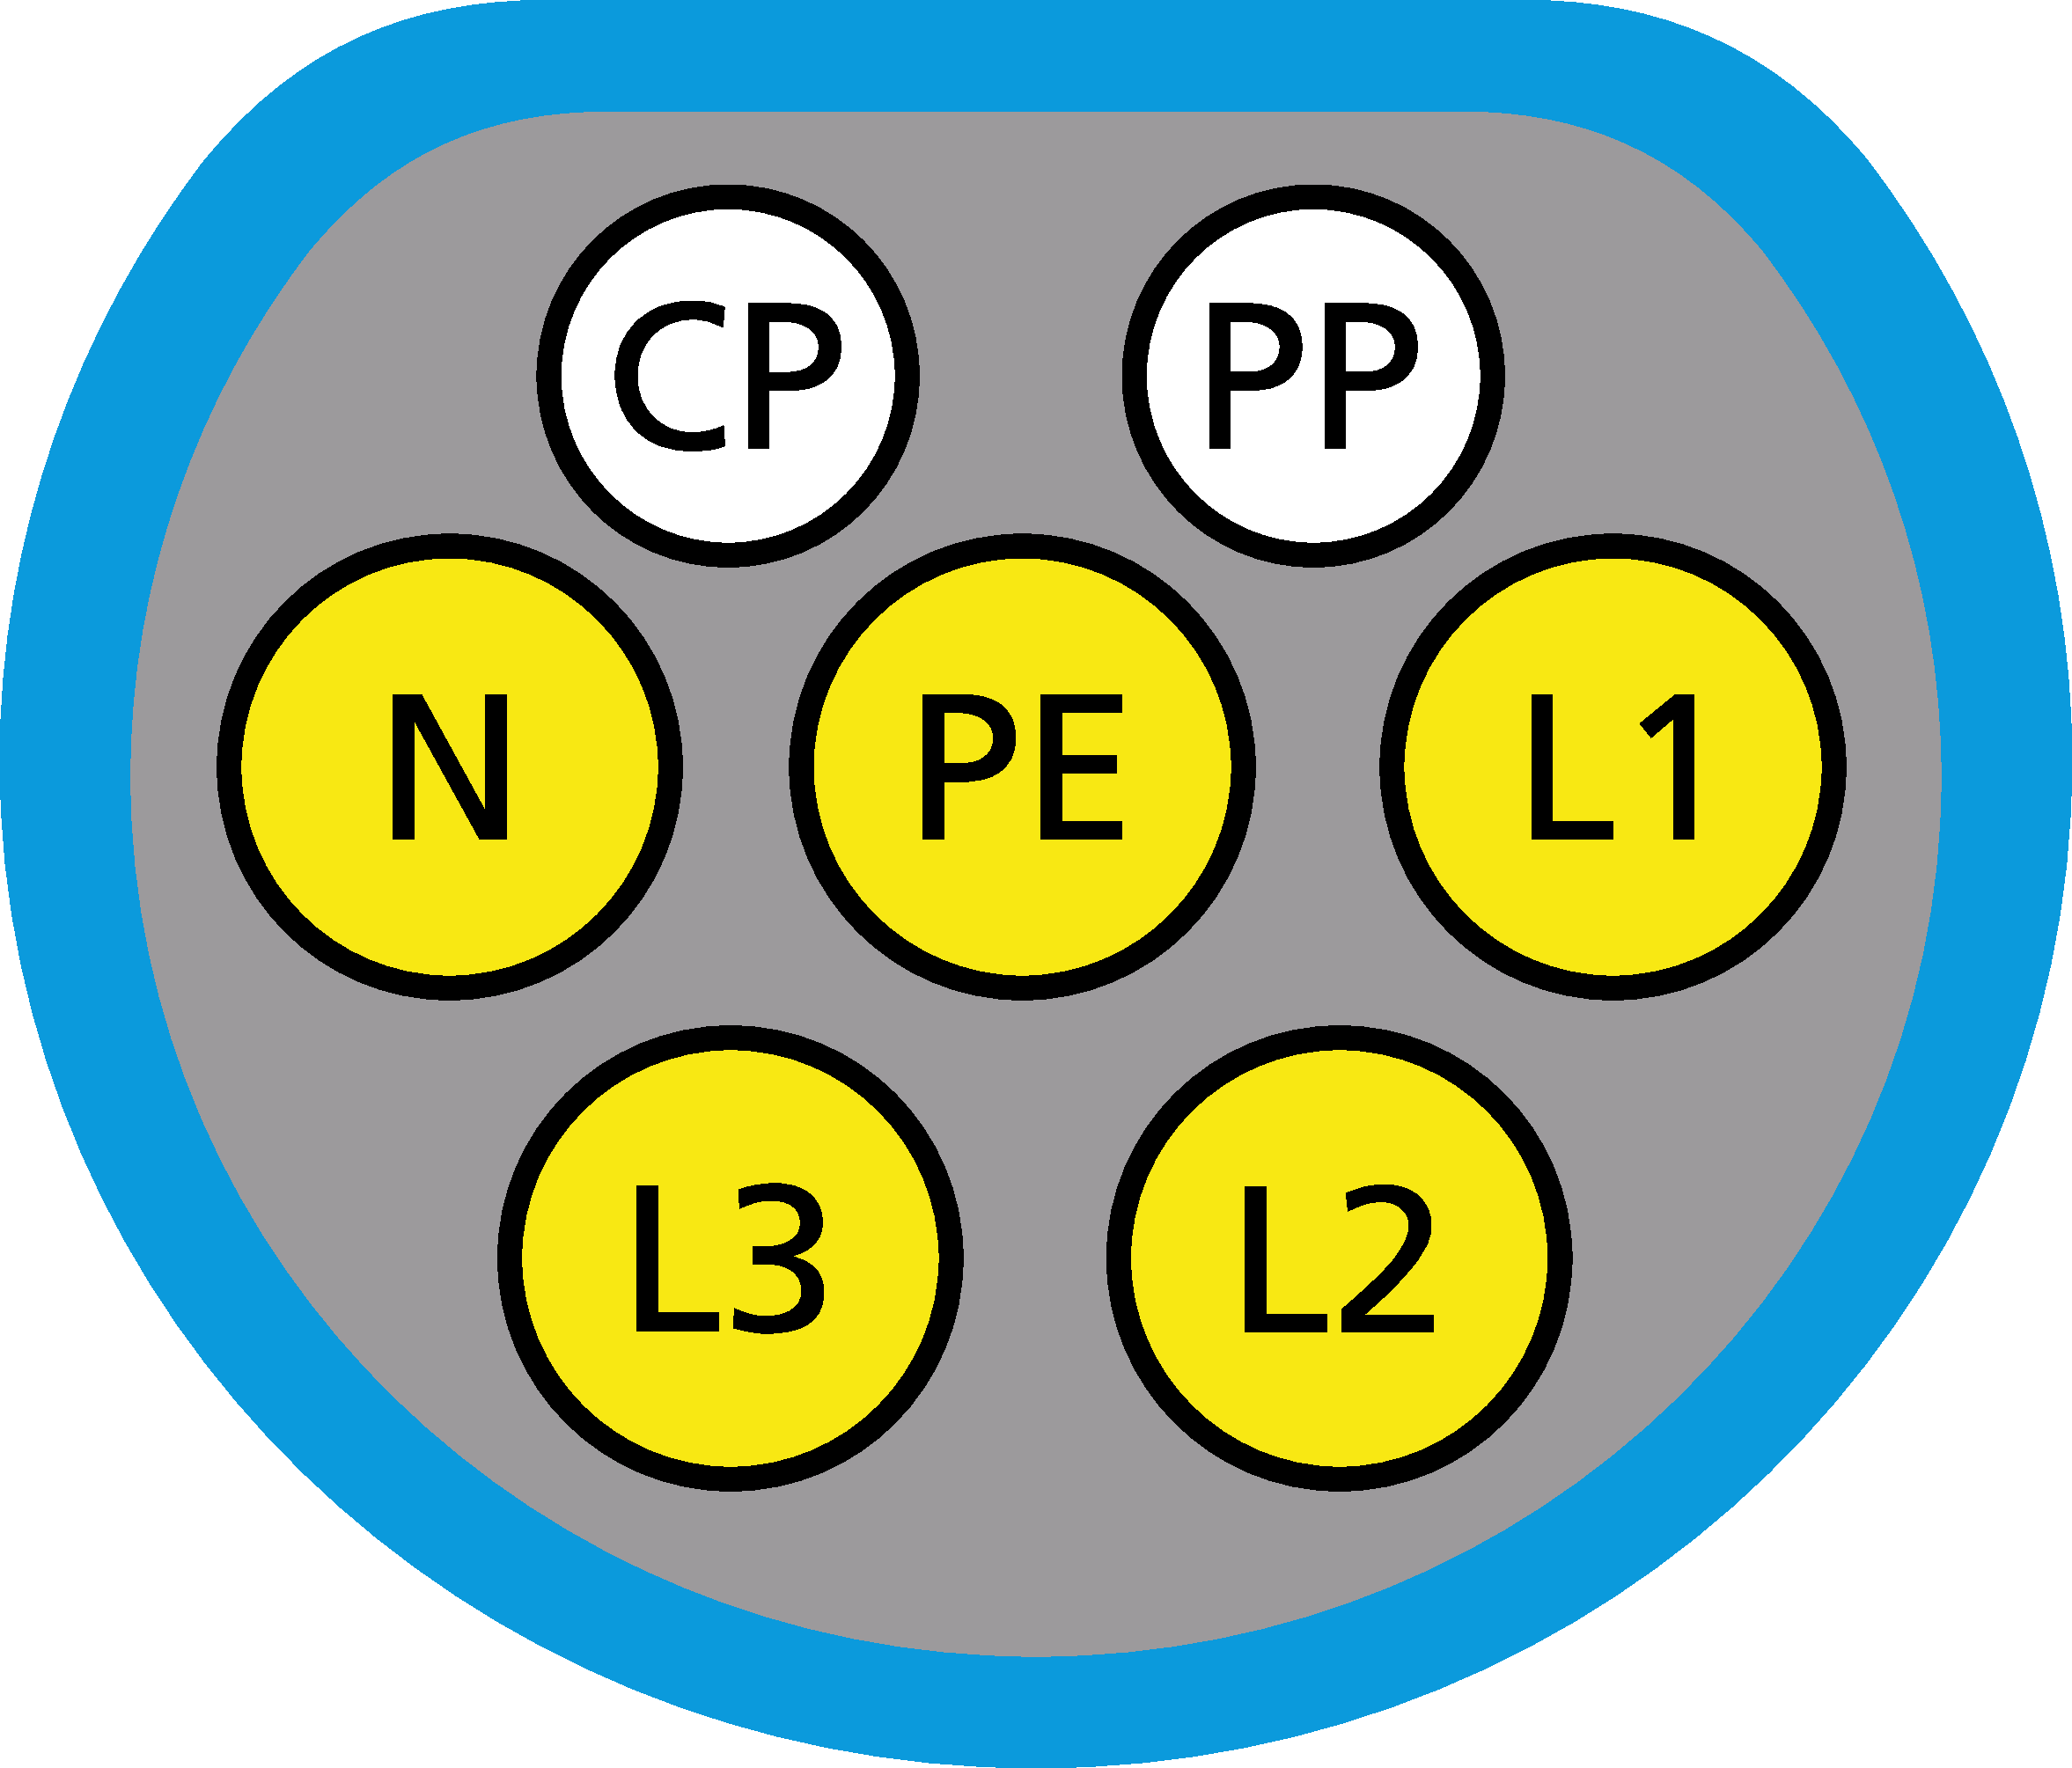
\includegraphics[width=.2\textwidth]{graphs/type2.pdf}
        %\caption{IEC 62196 Type 2 connector schematic}
        \label{fig:type2}
    \end{subfigure}
    \hfill
    \begin{subfigure}
        \centering
        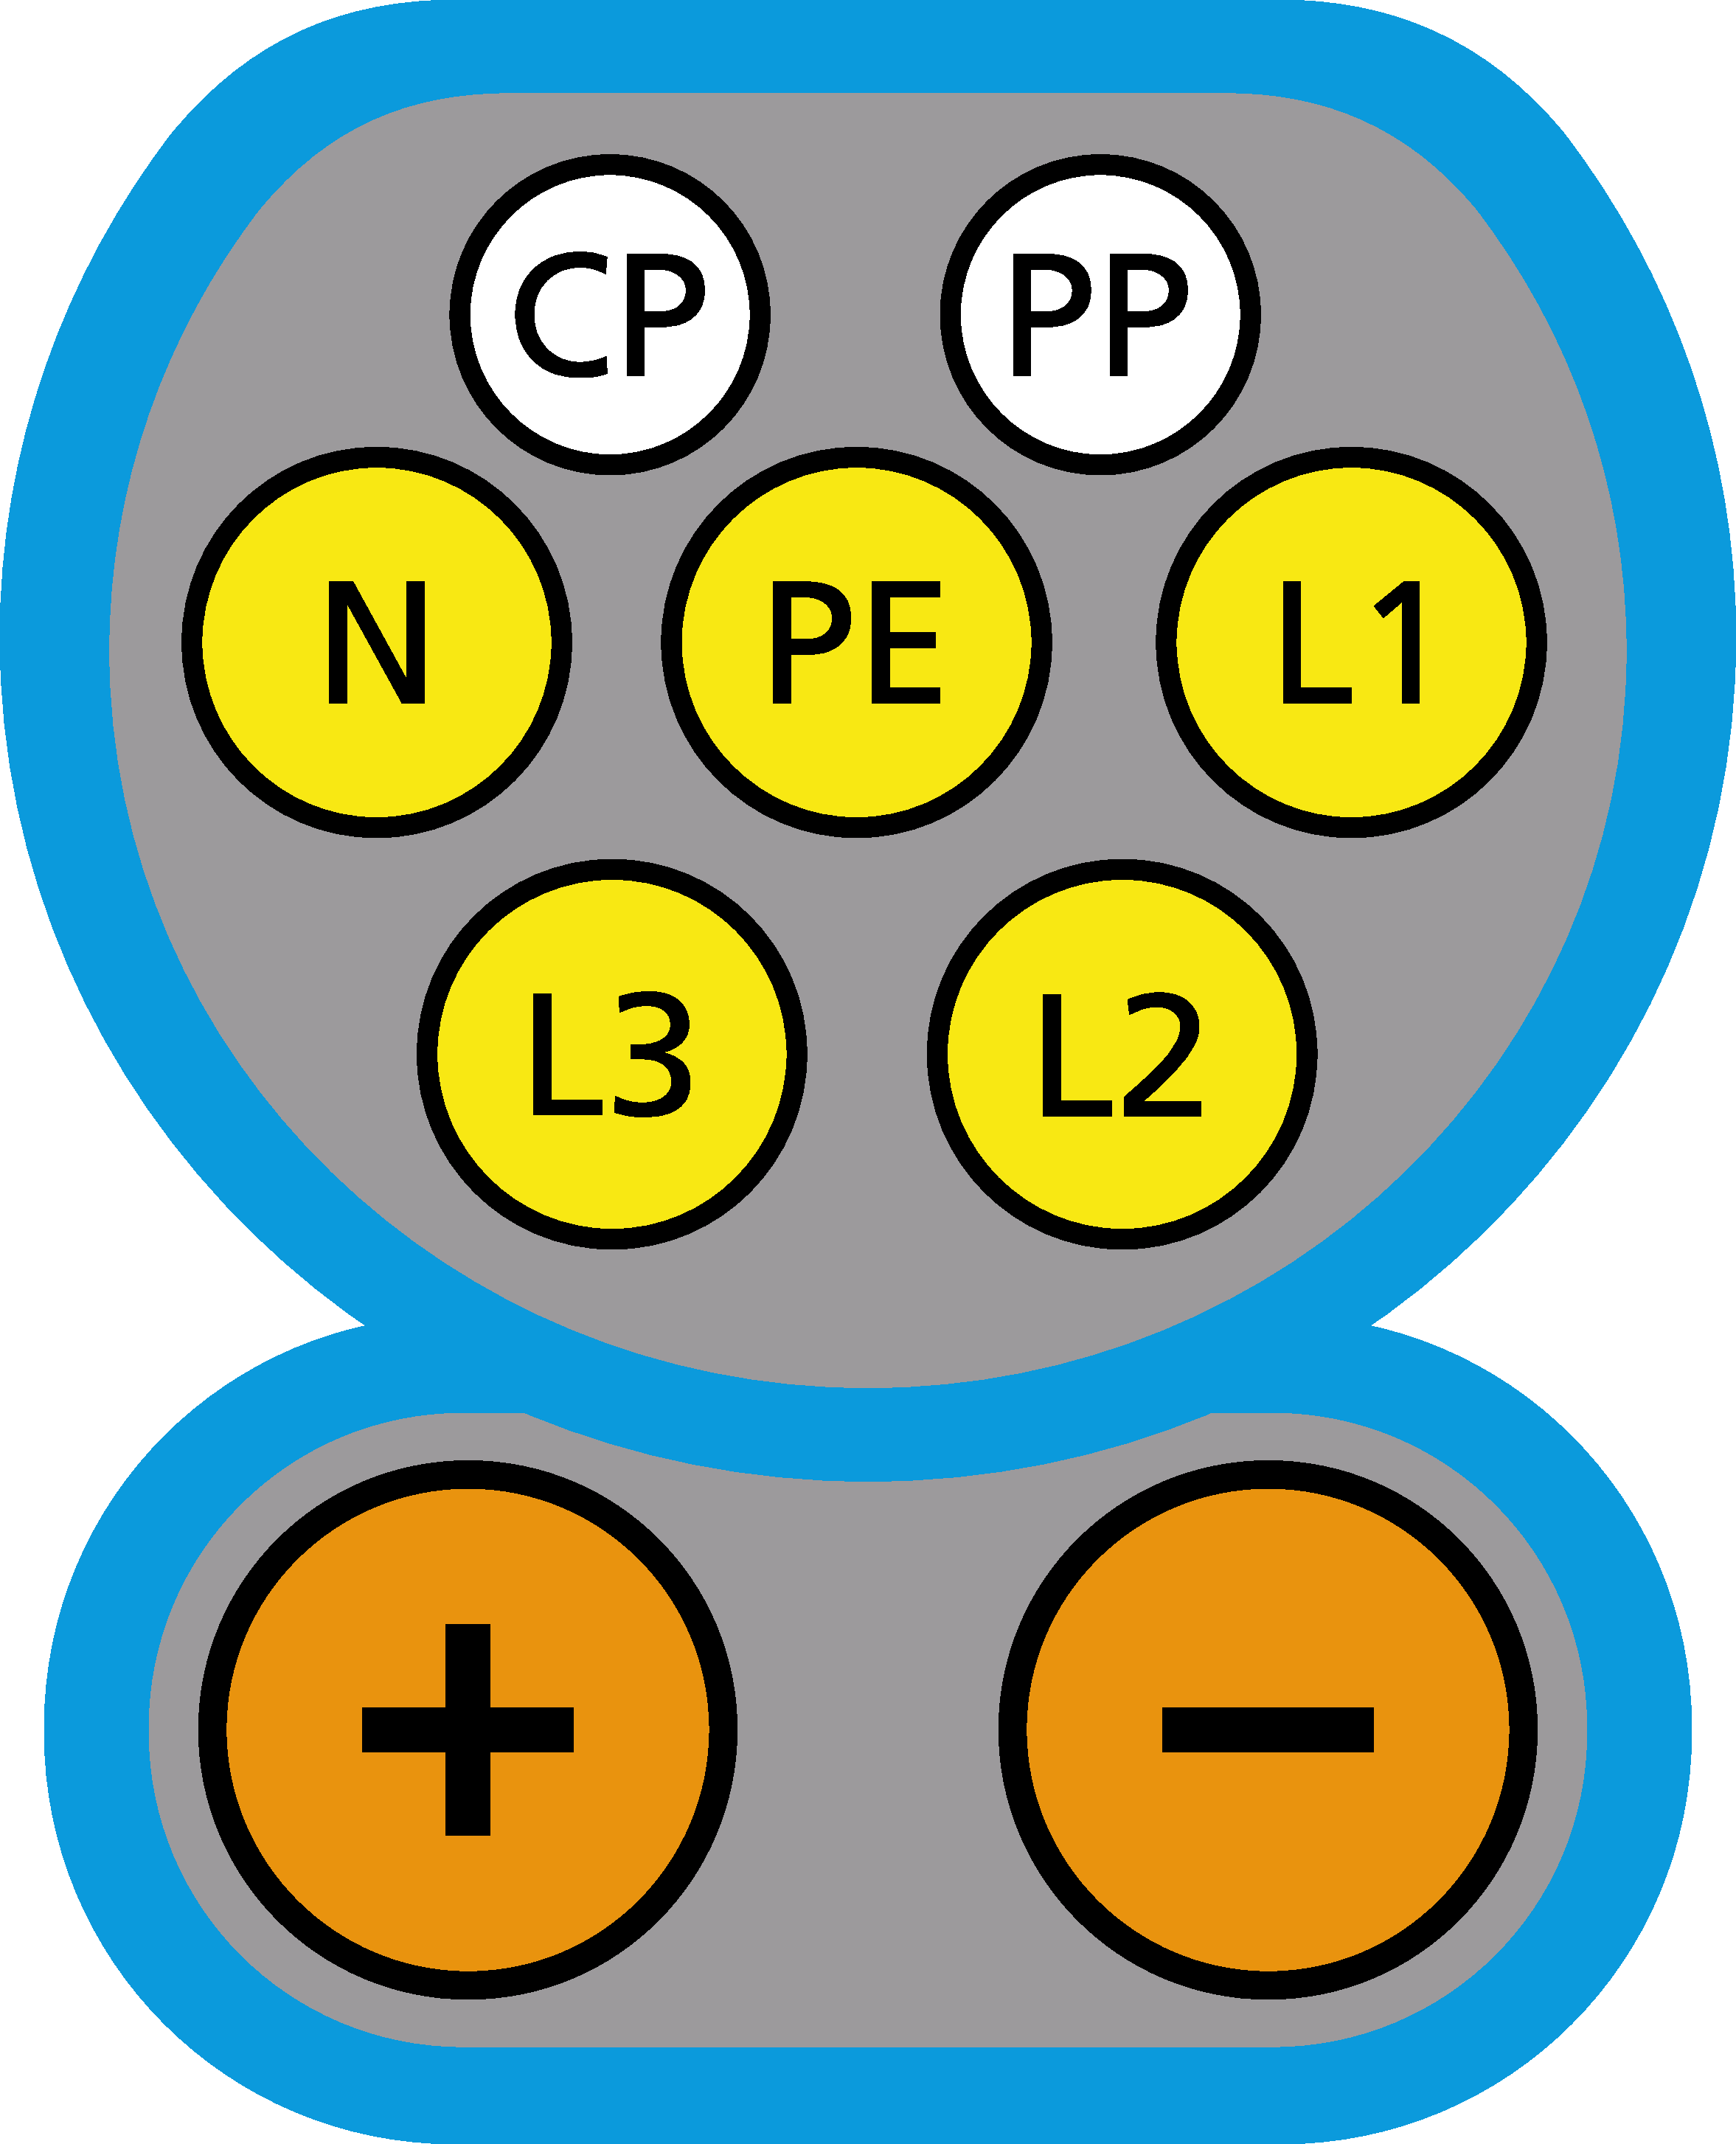
\includegraphics[width=.2\textwidth]{graphs/ccs.pdf}
        %\subcaption{Combined charging system connector schematic}
        \label{fig:ccs}
    \end{subfigure}
    \caption{Schematic diagrams type 2 (left) and combined charging system (right) connectors \cite{chris828_type_2020}}
    \label{fig:connectors}
\end{figure}

\subsection{High Level Communication} \label{sec:highlevelcomm}
While charging a vehicle with AC requires little to no communication,
DC charging stations on the other hand are required to communicate to the vehicle for properly supplying the correct voltage and power to the battery.
For this high level communication the industry standard ISO15118 \cite{isoiec_isoiec_2012} was created, enabling interoperability between different vehicle manufacturers and charging station vendors.
The standard is based on more or less common standards for all layers of the OSI model:
After the initial handshake of the low level communication, described in the previous section, is done, the charging station signals the vehicle to use high level communication by supplying a PWM duty cycle of 5\%.
Afterwards a powerline communication is modulated on top of the PWM signal between the charge pilot and protective earth.
To prevent crosstalk problems \cite{li_crosstalk_2019, theethayi_parameters_2003, ngo_bisse_crosstalk_2023} usually arising with powerline communication, ISO15118-3 \cite{isoiec_isoiec_2012-1} describes \enquote{signal level attentuation characterization} (SLAC).
SLAC measures the interference on the powerline communication line as well as matches vehicles with their nearest charging station connected to the powerline.
Once powerline communication is established, IPv6 with link-local stateless autoconfigured addresses is used on top for communication between the charging station and the vehicle.
While the ISO15118-2 standard \cite{isoiec_isoiec_2012} itself is based on TCP, first a UDP broadcast service discovery is used for exchanging IPv6 addresses as well as the port to connect to.
Through this TCP connection the actual payloads required for starting a charging session and controlling charging limits is performed.
For encoding payloads on this TCP connection the standard defines a \enquote{vehicle to grid transfer protocol} (V2GTP) packet format, which apart from some metadata contains one large payload blob encoded in the \enquote{efficient XML interchange} (EXI) format. \\
The ISO15118-2 standard defines a list of request messages sent from the vehicle to the charging station and corresponding response messages sent from the charging station to the vehicle.
During charging two packets are used repeatedly: \verb'CurrentDemandReq' and \verb'CurrentDemandRes'.
The first one is sent by the vehicle to request a specific voltage and current flowing into the vehicles battery.
The latter one is sent by the charging station informing the vehicle about currently measured voltage and current as well as the charging stations limits.
For example the car might request a voltage of $369V$ and a maximum current of $400A$ resulting in a desired charging power of $148kW$.
While the voltage has to be met, depending on the charging stations maximum output power the current might be lower than the requested value, resulting in a slower charging speed. \\
Before this main charge loop is started, the vehicle and charging station perform a payment and cable checking and precharging procedure.
Before the vehicle closes the main contactor relay between battery and charge port, the precharging procedure makes sure the voltage present at the cable matches the battery voltage, reducing in rush current and reducing wear on the main contactor relay.
For payment the vehicle first asks the charging station for supported payment methods.
As of today, mostly the \verb'external' payment method is used, which requires the user to pay through an app or contactless payments.
The standard also supports certificate based authentication allowing the car to authenticate itself and start charging directly after the cable has been plugged in.
This use case and its security implications will be covered in the next section.

\begin{figure*}[ht]
    \centering
    \begin{subfigure}
        \centering
        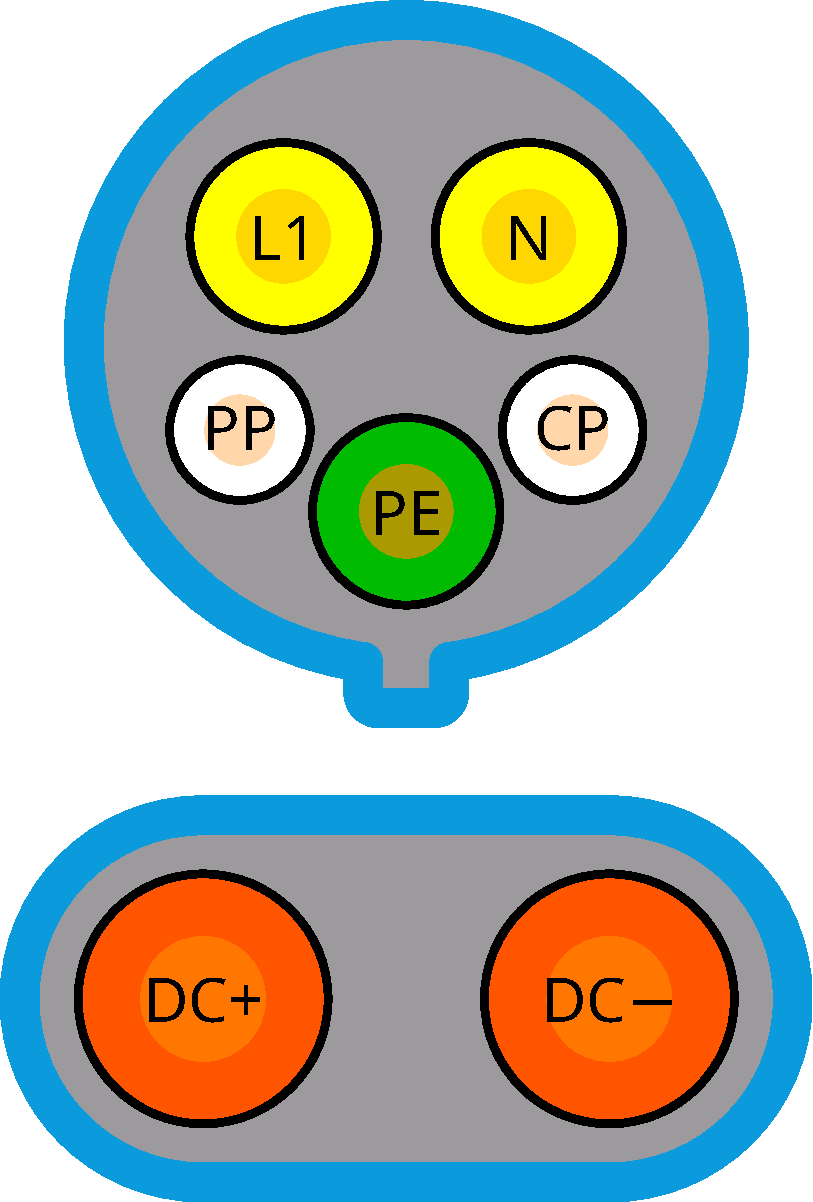
\includegraphics[width=.17\textwidth]{graphs/type1-ccs}
        %\caption{IEC 62196 Type 2 connector schematic}
        \label{fig:type2}
    \end{subfigure}
    \hfill
    \begin{subfigure}
        \centering
        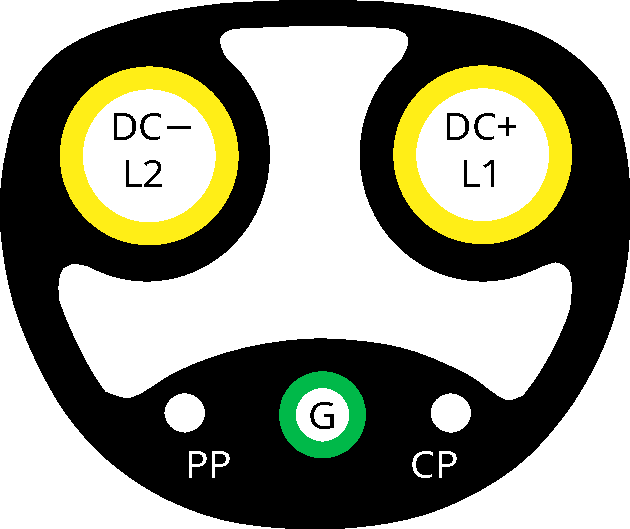
\includegraphics[width=.17\textwidth]{graphs/nacs}
        %\subcaption{Combined charging system connector schematic}
        \label{fig:ccs}
    \end{subfigure}
    \hfill
    \begin{subfigure}
        \centering
        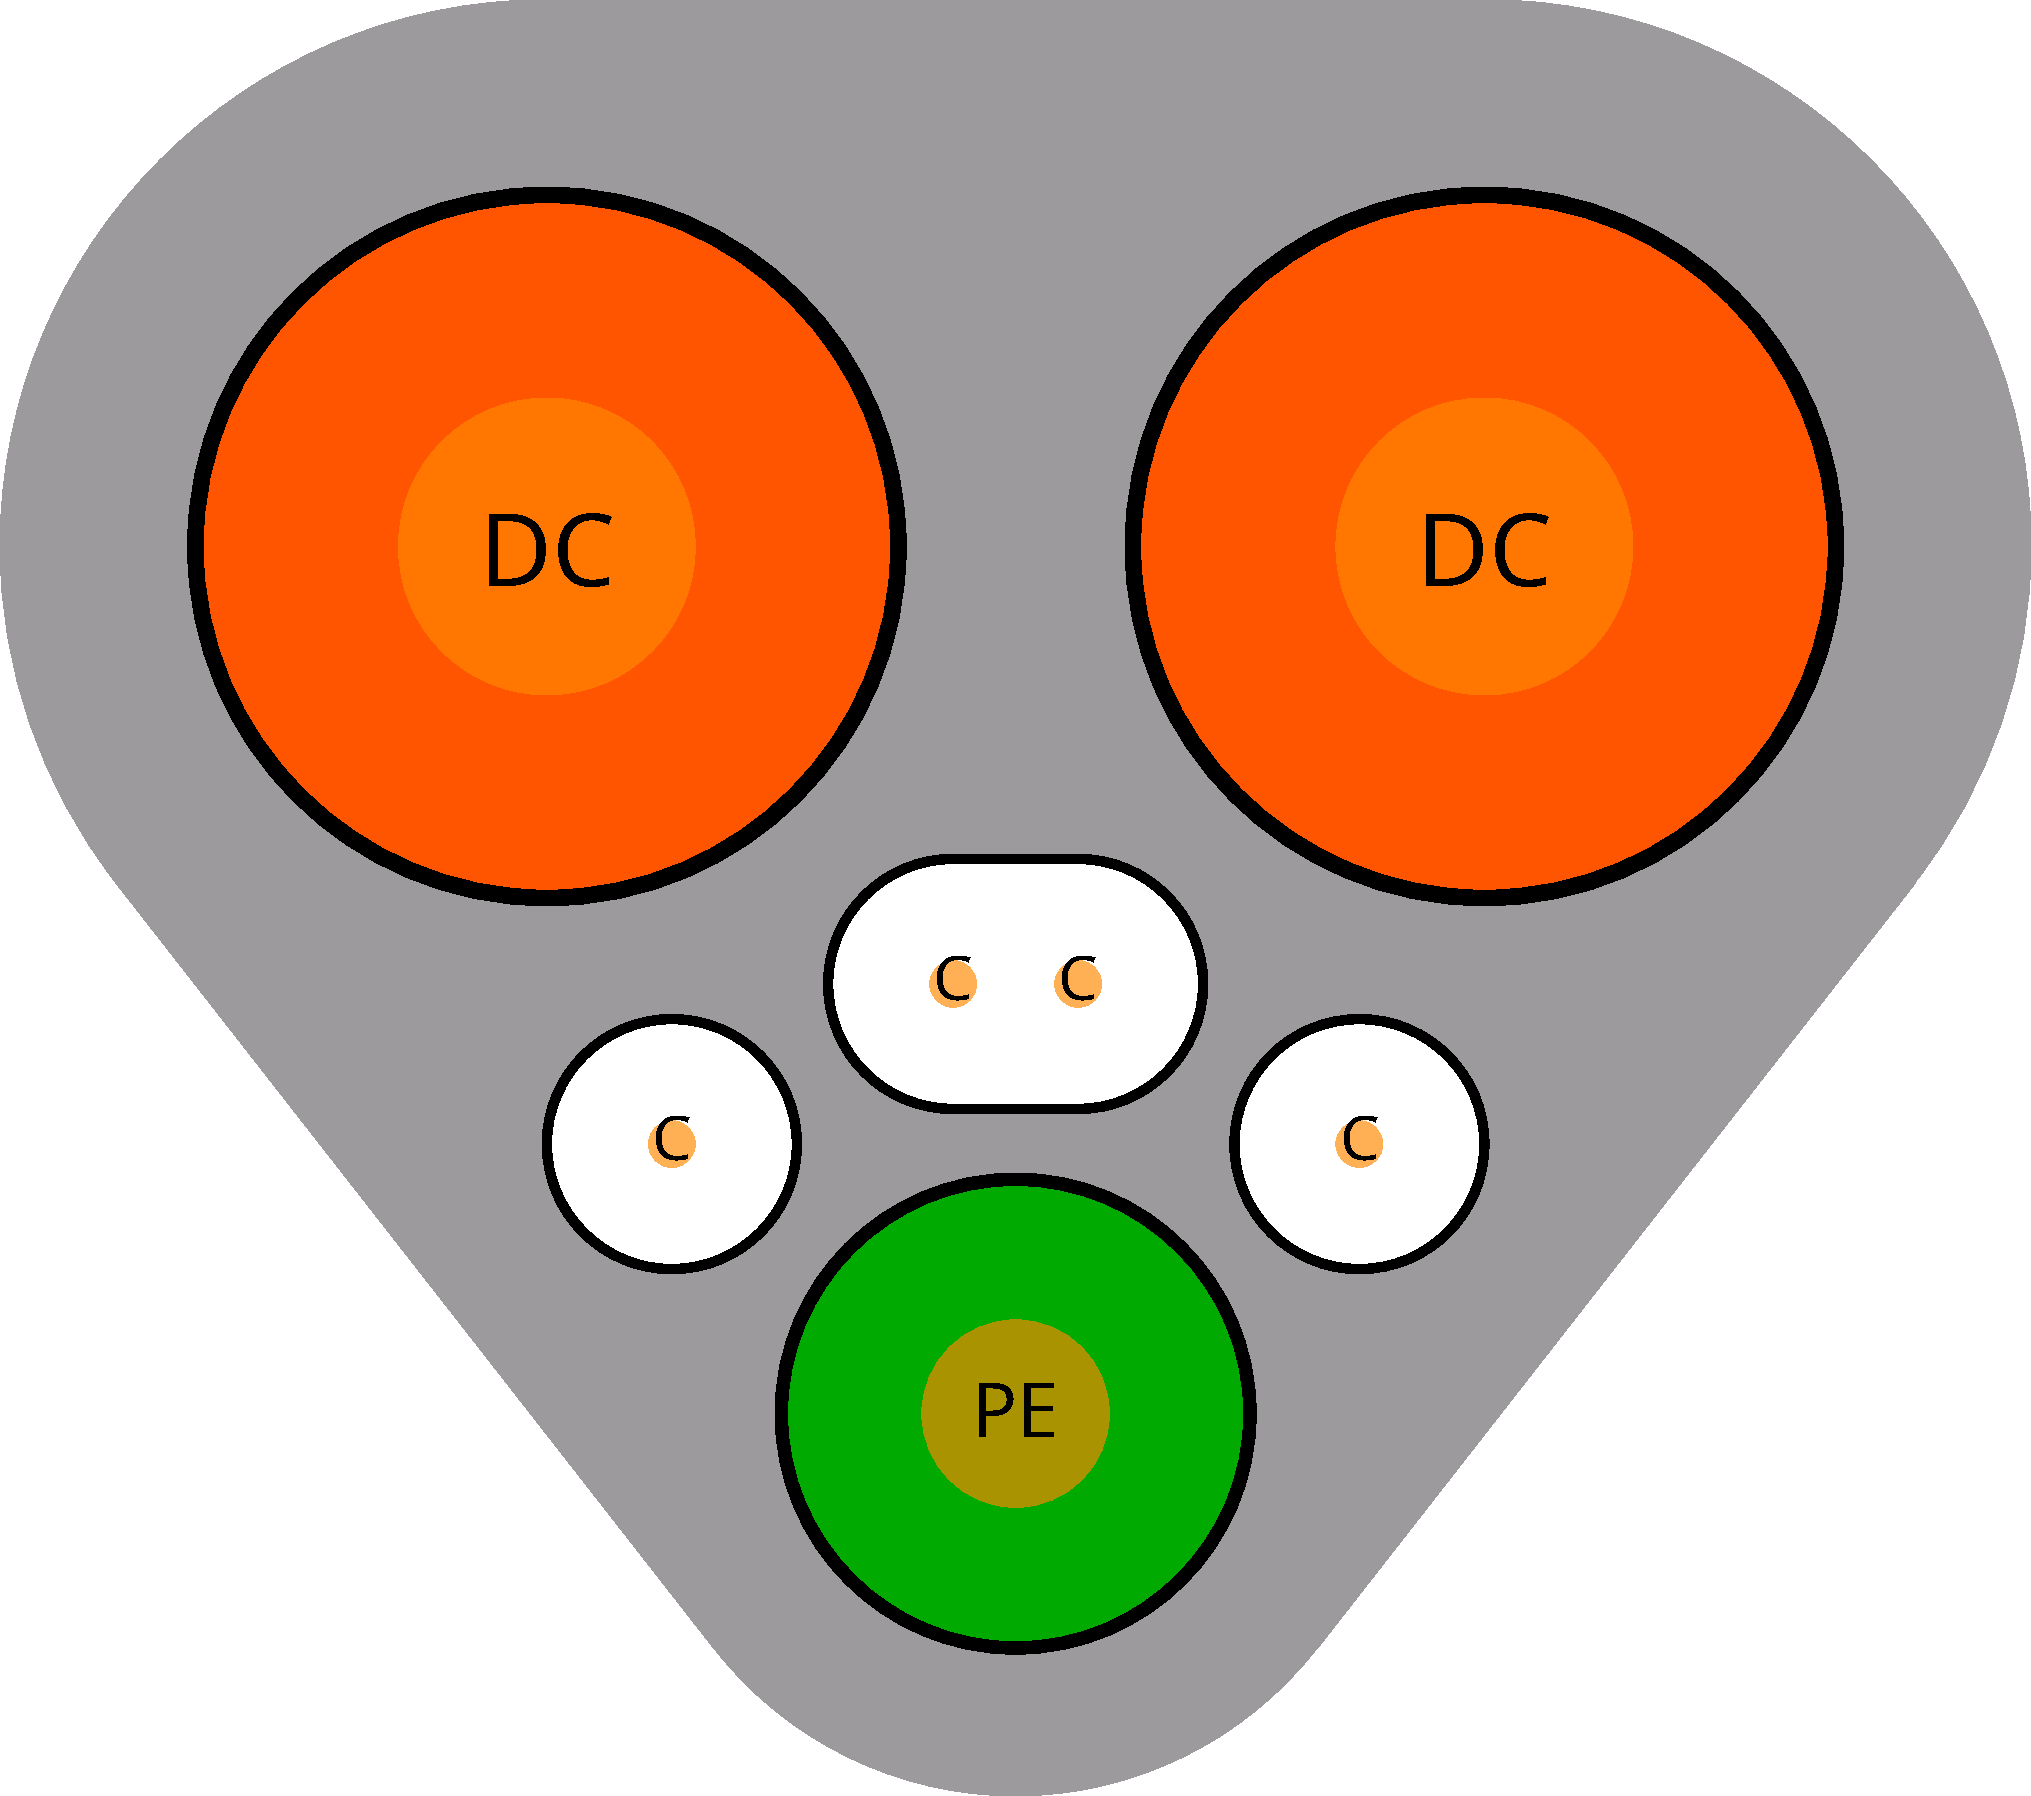
\includegraphics[width=.17\textwidth]{graphs/mcs}
        %\subcaption{Combined charging system connector schematic}
        \label{fig:ccs}
    \end{subfigure}
    \hfill
    \begin{subfigure}
        \centering
        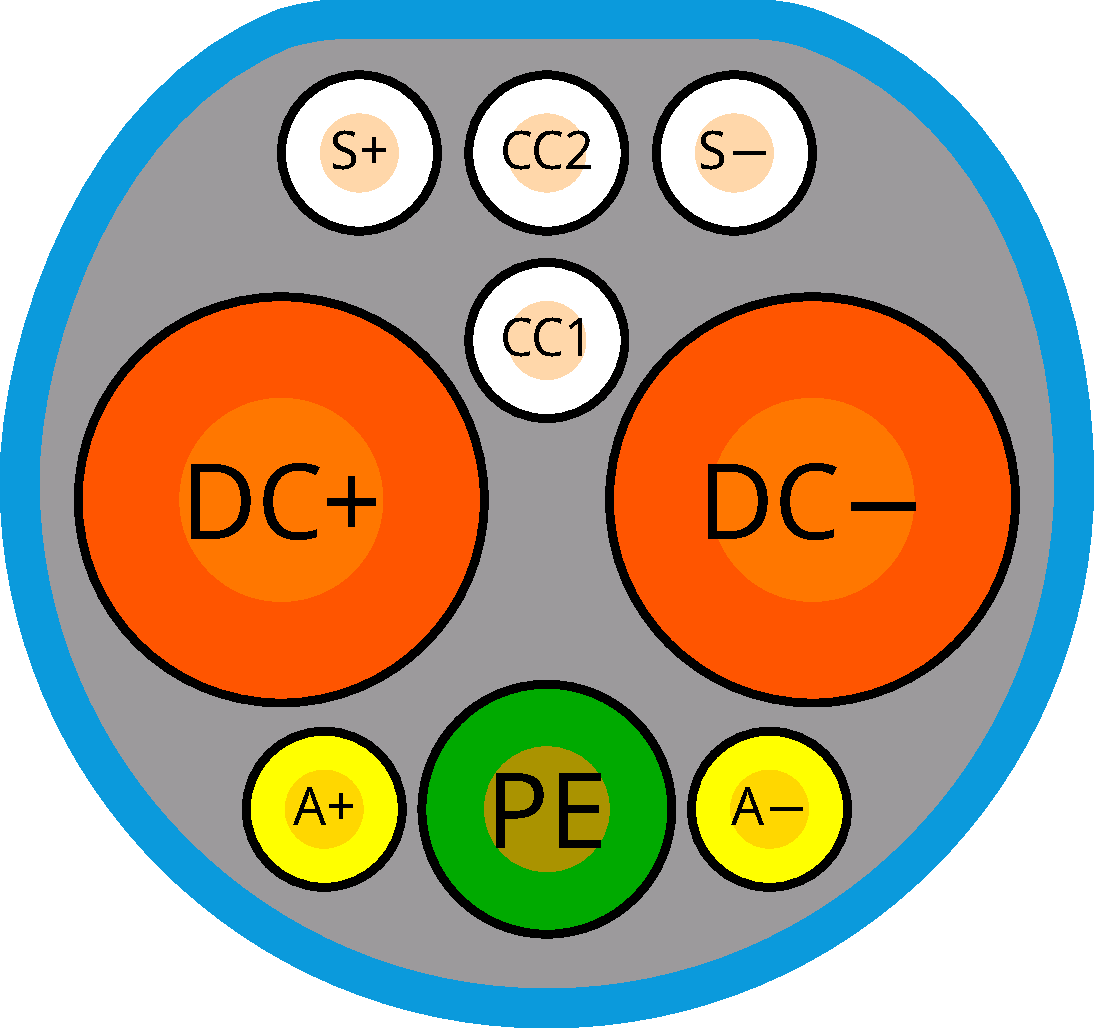
\includegraphics[width=.17\textwidth]{graphs/gbt}
        %\subcaption{Combined charging system connector schematic}
        \label{fig:ccs}
    \end{subfigure}
    \hfill
    \begin{subfigure}
        \centering
        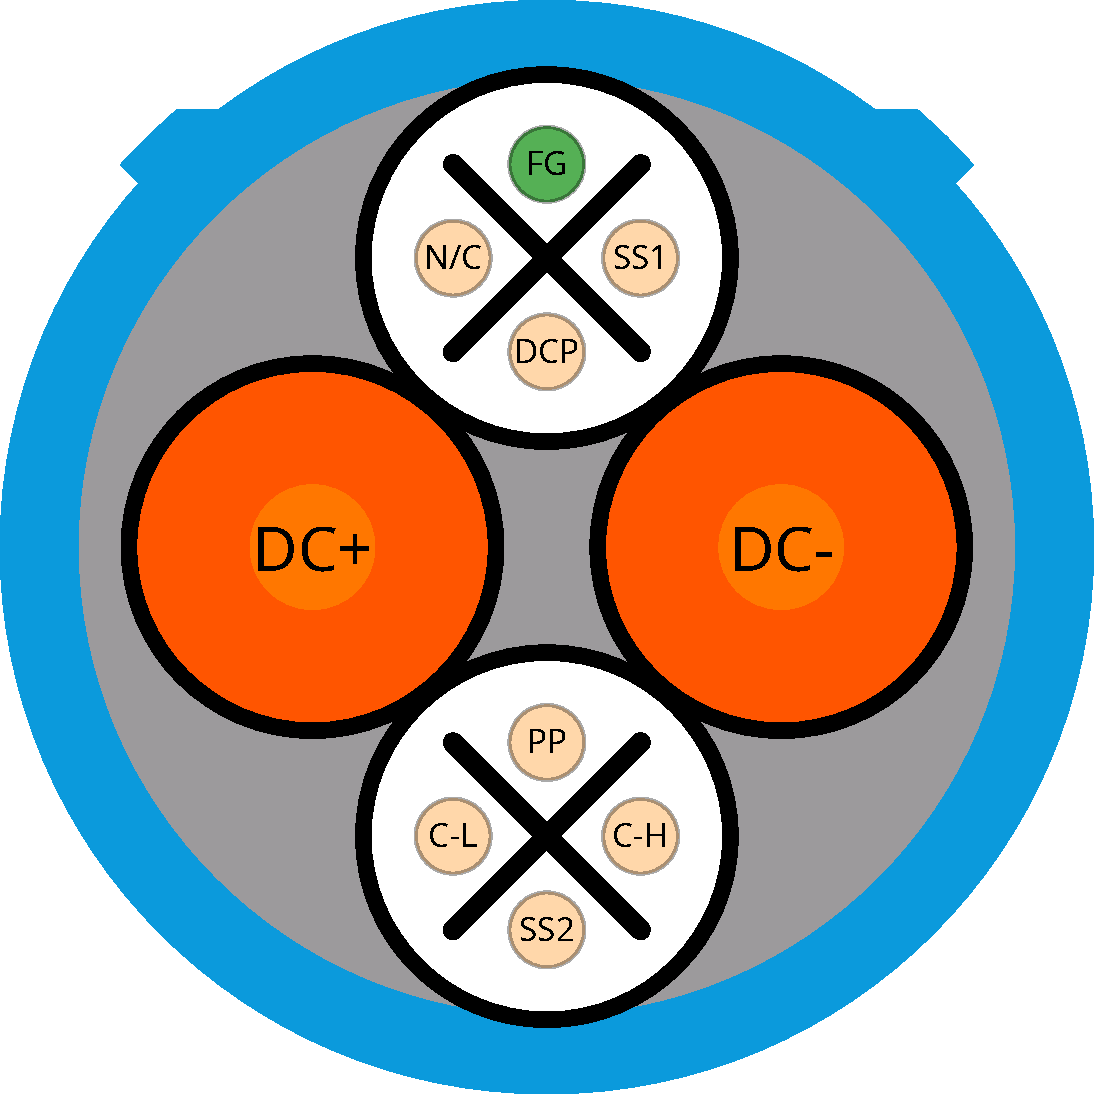
\includegraphics[width=.17\textwidth]{graphs/chademo}
        %\subcaption{Combined charging system connector schematic}
        \label{fig:ccs}
    \end{subfigure}
    \caption{Schematic diagrams of other fast charging connectors. From left to right: Type 1 CCS \cite{mliu92_drawing_2021}, NACS \cite{rickycourtney_drawing_2023}, MCS \cite{mliu92_speculative_2022}, GB-T \cite{mliu92_gbt-202343_2021}, Chademo \cite{mliu92_chademo_2021}}
    \label{fig:connectors}
\end{figure*}

% CCS1: By Mliu92 - Own work, CC BY-SA 4.0, https://commons.wikimedia.org/w/index.php?curid=108177318
% NACS: By RickyCourtney - Own work, CC BY-SA 4.0, https://commons.wikimedia.org/w/index.php?curid=133111353
% MCS: By Mliu92 - Own work, CC BY-SA 4.0, https://commons.wikimedia.org/w/index.php?curid=119080953
% GB/T: By Mliu92 - Own work, CC BY-SA 4.0, https://commons.wikimedia.org/w/index.php?curid=108206603
% chademo: By Mliu92 - Own work, CC BY-SA 4.0, https://commons.wikimedia.org/w/index.php?curid=108209697

\subsection{ISO15118 Security Concepts} \label{sec:iso15118tls}
While the most commonly used scheme for the charge loop communication is based on plain TCP, the ISO15118 standard also allows to use TLS for encrypted communication.
Using the UDP broadcast packet, the vehicle can signal support for TLS encrypted communication.
If the charging station also supports TLS encryption it signals this to the vehicle in the UDP response including a port to connect to using TLS.
While TLS provides a secure way of communication, in order to handle authentication it requires a private key infrastructure (PKI) to sign and distribute certificates.
ISO15118 describes a potential layout of this PKI handing out certificates to vehicle manufacturers and charge point operators, but does not name a specific entity managing this PKI.



\subsection{Other Communication Standards}
While Type 2 and CCS are the most used plugs for passanger cars in europe, there do exist some other plugs and charging standards for fast charging battery electric vehicles.
In total there are five other major plugs used for fast charging around the globe, listed below and shown schematically in \ref{fig:connectors}:

\begin{enumerate}
\item GB/T charging standard used in China
\item CHAdeMO used in Japan
\item Type 1 CCS formerly used in North America
\item NACS future north american charging standard
\item Megawatt charging system (MCS)
\end{enumerate}

While europe has the type 2 connector for three phase AC charging, america uses a different connector called type 1, since their power grid is usually not based on three phases.
There exists a type 1 CCS connector, adding two pins for DC charging, similarly to type 2 CCS.
Since communication is identical they can both be referred to as \enquote{CCS connectors}, or specified as \enquote{CCS1 connector} for the american version and \enquote{CCS2 connector} for the european version.
Similarly the megawatt charging system is also based on ISO15118, but uses a different connector, allowing higher currents and thus faster charging intended for trucks ans buses.
After Tesla open sourced their proprietary connector in 2022 \cite{noauthor_opening_nodate} it became quickly adopted by car manufacturers and charging station operators.
While its socket is different, it is also based on ISO15118 communication described above. \\
GB/T and CHAdeMO are the charging standards used in China and Japan respectively.
They use CAN bus for communication rather than powerline making their implementation easier and cheaper, while disallowing advanced use cases ISO15118 provides.
Since EV sales are much higher in Asia than in Europe and North America \cite{noauthor_trends_nodate}, the worldwide market share of vehicles with GB/T and CHAdeMO sockets remains significant nevertheless their usage only in China and Japan.
According to Blech \cite{blech_project_nodate} at the end of 2019 the combined market share of GB/T and CHAdeMO was 55\%. Figure \ref{fig:connector_marketshare} shows the market share of all connectors.

\begin{figure}[ht]
    \centering
    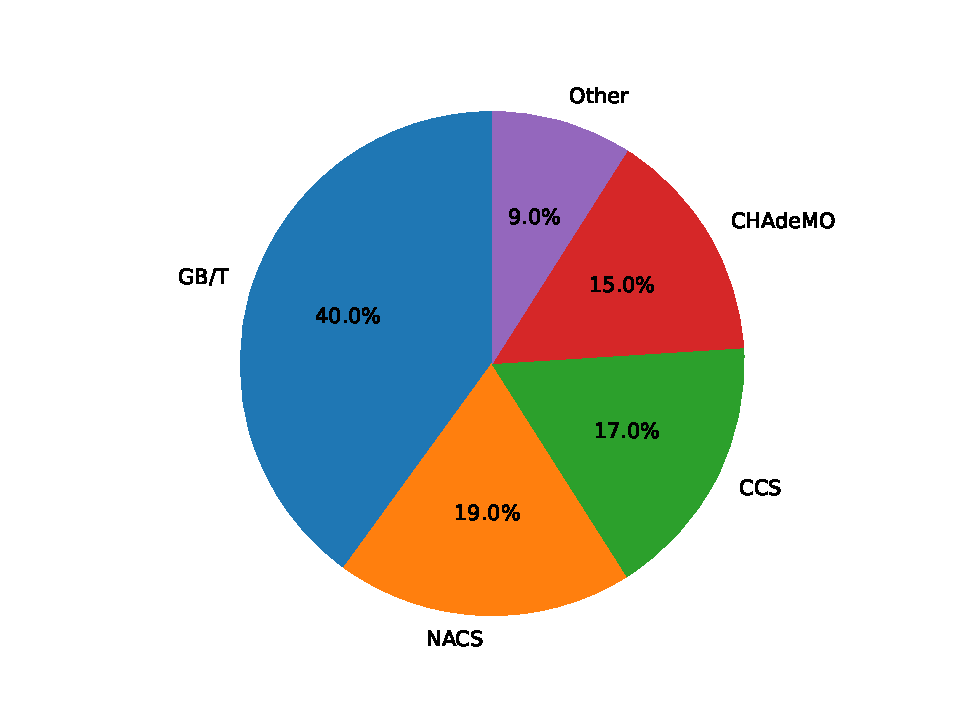
\includegraphics[width=.489\textwidth]{graphs/worldwide_plugs.pdf}
    \caption{Charging socket market share at the end of 2019, based on Blech \cite{blech_project_nodate}}
    \label{fig:connector_marketshare}
\end{figure}

%% \cite{garofalaki_electric_2022} - OCPP security issues and challenges



\section{Charging Station Vendors}
\begin{figure}[ht]
    \centering
    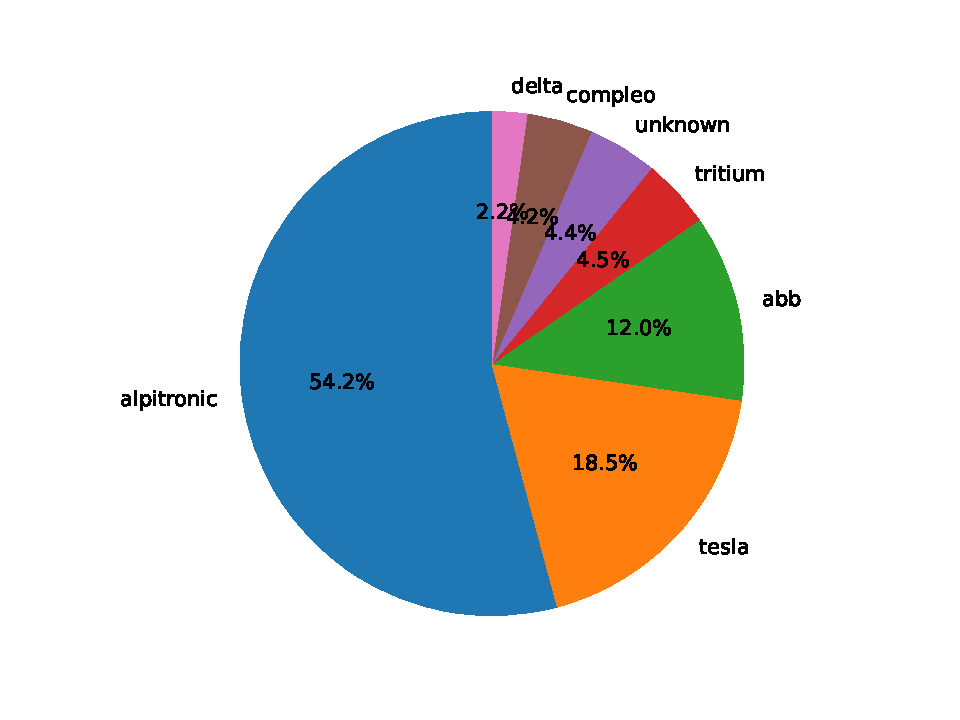
\includegraphics[width=.489\textwidth]{graphs/market_analysis.pdf}
    \caption{DC charging station vendor market share in Germany}
    \label{fig:marketshare}
\end{figure}

After the standardization of the type 2 connector in 2009 and even after the introduction of CCS in 2014 most charging stations built offered only AC charging.
Since AC charging stations include mostly components commonly found in home and industrial electric installations, companies active in the field of electric components and installations, such as Mennekes, Hager and E.ON, started building AC charging stations \cite{dalheimer_ladeinfrastruktur_2017}. \\
After CCS connectors became more popular in electric vehicles and the demand for high power fast charging grew \cite{das_electric_2020}, some companies started developing and producing DC fast charging stations.
While AC charging stations rely on simple components, DC charging stations are more complex, incorporating AC to DC conversion, high level communication and cooling equipment.
While the market of AC charging station manufacturers is quite diverse, the complexity of DC charging causes only a handful of companies to produce significant numbers of high power charging stations. \\
As a part of this research we analyzed the current market share of DC charging stations in Germany.
% TODO: make goingelectric.de a reference
The largest registry of charging stations in Germany and Europe is \url{goingelectric.de}. This community led effort manages an interactive map as well as an API to fetch positions and metadata for each charging point.
Using the manufacturer and model information included in the goingelectric database, allows to analyze DC charging station market share.
% TODO: extend methodology of scraping
With currently over 6000 DC charging points Alpitronic manufactured over 50\% of todays DC charging stations in Germany.
Second place is Tesla with its own supercharger devices and self managed charging network making up 18.5\%.
ABB is the only traditional electric installation company active not only in the AC charging station market, but also producing DC charging stations, making up 12.0\% of all DC charging stations currently installed in Germany.
With only three other companies having above 1\% market share and Tesla not selling to third parties, the current DC charging station market is dominated by Alpitronic leaving behind well known companies like Siemens, Volkswagen and Porsche Engineering below the 1\% mark.
Figure \ref{fig:marketshare} shows the market share of all manufacturers currently used in Germany, which have more than 1\% market share.

\iffalse
% TODO: add text about charging sockets and their market share / probability
\begin{figure}[ht]
    \centering
    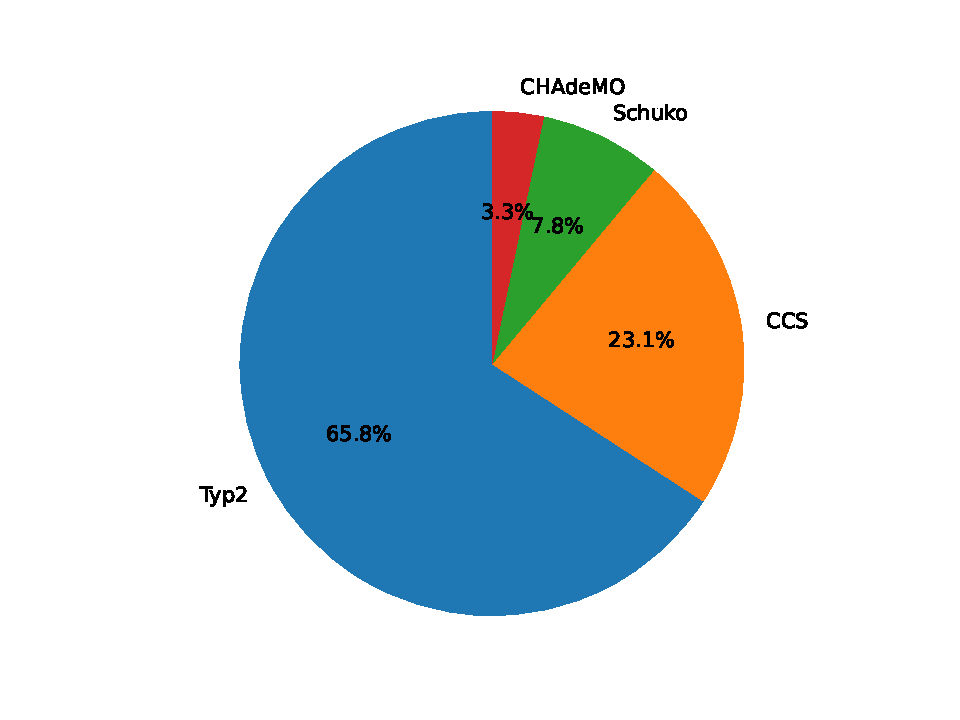
\includegraphics[width=.489\textwidth]{graphs/socket_analysis.pdf}
    \caption{Charging station socket market share}
    \label{fig:sockets}
\end{figure}

\begin{figure}[ht]
    \centering
    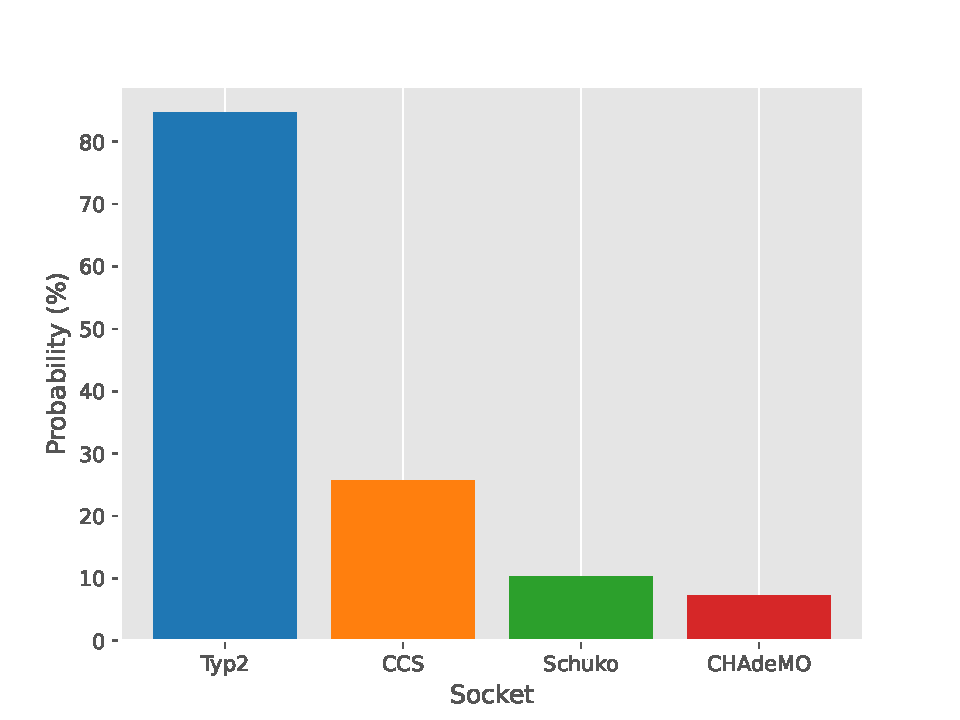
\includegraphics[width=.489\textwidth]{graphs/socket_probability.pdf}
    \caption{Probability to find socket X at a random charging location}
    \label{fig:socketsprob}
\end{figure}
\fi



\section{Charging Station Architectures}
While the interface between vehicle and charging station as well as the interface between charging station and grid is standardized, the conversion process from AC grid power to DC grid power is not.
Other research has already extensively covered different approaches towards AC to DC conversion and their attributes in regard to battery charging \cite{tu_extreme_2019, das_electric_2020, deb_review_2021}.
While the details of high power electronics are hardly relevant to this cybersecurity review, it is important to note the two main architecture approaches and their impact on communication mechanisms within a charging station.
The following factors play a role when designing a charging station architecture:
\begin{itemize}
    \item Electric batteries cannot be charged with the same speed for the entire charging cycle.
    Especially when the battery is low or nearly full, the charge speed has to be decreased in order to minimize battery degrading.
    Todays electric vehicles usually have a power peak between 20\% and 40\% state of charge.
    Before and afterwards the charging power and thus the charging speed is decreased significantly.
    \item When building up DC chargers, one site is usually equipped with more than just one charging station. Instead, multiple charging stations are combined to a larger charging park.
    \item Because electricity pricing is based on peak power draw from the grid, charging park operators often reduce peak power drain using stationary battery storage.
    \item Charge parks are often combined with solar providing roofing and additionally decreasing energy drain from the grid.
\end{itemize}

\subsection{AC vs DC Bus architectures}
Taking these factors into consideration Deb et al. \cite{deb_review_2021} discuss two different approaches when building up charging parks: DC bus systems and AC bus systems.
In AC bus systems all devices in the charge park either produce energy feeding into the AC bus or consume energy from the AC bus.
Usually the AC bus is the regular energy grid, making this approach easy and cheap to implement, while allowing the use of a wide range of off the shelf solar and battery storage components. \\
In DC bus systems all devices in the charge park directly feed into a DC power line. Because both solar panels as well as batteries run on DC power this approach eliminates significant conversions losses when converting power from DC to AC and back.
Thus this approach promises higher efficiency and thus less operating cost it.
While AC solar inverters and battery storage solutions are commonly used in industrial and home applications, specialized DC solutions are not commonly available as of today, leading to DC bus architectures having a higher up front investment and complexity.

\subsection{Architectures in Use Today}
The investment and complexity hurdle discussed above, can be observed when analyzing the system architecture used by dominant charging station manufacturers mentioned in the previous section.
Alpitronic, ABB and Tritium all directly convert AC grid power to DC power for charging electric vehicles.
None of these manufacturers allow directly feeding in DC power into their charging stations.
They do however implement one remedy to decrease the impact of the dynamic charge speed of electric vehicles: Providing two charging sockets per charging station and performing load sharing between the two.
For example Alpitronic chargers contain two to four AC to DC power conversion modules.
When two cars are being charged at once, rather than statically assigning conversion modules to outlets, the modules are dynamically switched between outlets.
This switching allows the charge power to be distributed unevenly between both vehicles based the demand on each outlet, effectively increasing the maximum output per outlet without increasing the total amount of conversion modules. \\
While the first three generations of Tesla superchargers used a similar load sharing technique, the new v4 superchargers are the first DC bus based charging stations.
They feature larger conversion module converting AC grid power to DC and one DC to DC conversion module for each supercharger outlet.
One conversion module is placed per four superchargers, interconnecting the conversion modules using a DC bus at nearly 1000V. \\
With Tesla being a manufacturer of not only charging stations, but also solar and stationary battery storage solutions, they were the first to introduce a DC bus charging station system, possibly integrating solar and storage directly with the bus at a later stage.
With these kind of systems being more efficient and demand in vehicle charging steadily increasing, more manufacturers can be expected to develop similar systems in the future.

\subsection{Communication aspects of AC vs DC Bus systems}


% TODO write this section

%% \cite{acharya_cybersecurity_2020} - very good architecture schematic of grid/charging station/EV connections and communication.



\section{Attack Vectors and Impact}
There already exists some research regarding the security of charging stations. Most of them however focus either on high level risk assessments \cite{acharya_cybersecurity_2020, sanghvi_cybersecurity_2021, assi_ensuring_2023, mahrukh_load_2023, park_potential_2019, ahalawat_security_2022, bao_threat_2018} or target aspects of vehicle charging other than DC fast charging communication \cite{nasr_chargeprint_2023, sklyar_chargepoint_nodate, sarieddine_investigating_2023, nasr_large-scale_nodate, nasr_power_2022}.
The following subsection describes some of the few attacks successfully carried out against DC charging communications.
Afterwards general problems with implementing the security concepts defined in ISO15118.

\subsection{Attacks Against Charging Communication}

\subsection{ISO15118 Security Implementation}
As described in section \ref{sec:iso15118tls} the ISO15118 standard uses TLS for securing communication and even for payment authentication.
The standard however does not name a company or institute handing out certificates required for TLS communication.
As of today there are at least four different companies that created a PKI and allow third parties to acquire certificates \cite{charin_charin_nodate, hubject_download_nodate, nexusgroup_identities_nodate, irdeto_irdeto_nodate}.
Normally a certificate authority simply provides certificates for a service provider, for example for a website.
With ISO15118 however, the vehicle requires a matching client certificate for authenticating.
Thus while having multiple certificate authorities is generally a good idea, it creates a maintenance overhead for both vehicle manufacturers and charging station operators in order to support all authorities.
Because of this complexity, as of today the vast majority of all charging communication sessions is not encrypted at all.
Since TLS is required in order to use plug and charge, users have to use external payment menthods such as RFID cards or apps rather than PnC.
While PnC promises to improve usability and thus overall technology acceptance, the nature of the TLS implementation details set by the ISO15118 charging standard hinder its spread and is thus rarely used today.



\section{Conclusion}
As discussed in this paper, the market of both AC and DC charging stations is growing rapidly.
Even though DC fast charging stations come with additional security implications, cybersecurity has not been a focus of the charging station industry in the past, leading to many textbook vulnerabilities in charging infrastructure.
In the recent past this situation is starting to improve, with various institutions publishing guidelines and plans on securing charging infrastructure \cite{mccarthy_cybersecurity_2023, encs_security_nodate}. \\
While this is a step in the correct direction, a lot of low hanging fruits in regard to security research of DC charging stations remain untouched.
This is underlined by the fact, that most scientific publications covering cybersecurity of charging communication in general are purely theoretical.
While some AC charging stations and some web based services have been target of security research, little research has been done targeting real DC fast charging stations nor their communication with vehicles. \\
In future research our plan is to perform penetration testing on charging station communication implementations both manually and using automated pentesting techniques.
The goal of our future research will be to not only identify vulnerabilities in implementations, but also identifying general problems with the ISO15118 standard.
One promising approach we are currently working on is to use state of the art fuzzing techniques for automatically identifying edge cases in the protocol and its implementations.

\section*{Acknowledgment}

This work was created in the research project eSiLa funded by the Bavarian Ministry of Economic Affairs, Regional Development and Energy under grant DIK0512/01.

% TODO fix URL only references looking weird
% TODO fix overflowing URLs
\printbibliography
\end{document}
